\chapter{Tutorial: Processing Mars Orbiter Camera Imagery}
\label{ch:moc_tutorial}

\definecolor{lgray}{gray}{0.95}

\section{Quick Start}

The Stereo Pipeline package contains command-line programs that
convert a stereo pair in ISIS {\em cube} format into a 3D ``point
cloud'' image: \texttt{\textit{stereo-output}-PC.tif}.  This is an
intermediate format that can be passed along to one of several
programs that convert a point cloud into a mesh for 3D viewing or a
gridded digital elevation model (DEM) for GIS purposes.

There are a number of ways to fine-tune parameters and analyze the
results, but ultimately this software suite takes images and builds
models in a mostly automatic way.  To create a point cloud file, you
simply pass two image files to the \texttt{stereo} command:

\begin{verbatim}
  ISIS 3> stereo left_input_image right_input_image stereo-output
\end{verbatim}

See section \ref{running-stereo} for a more detailed discussion. 
 
You can then make a visualizable mesh or a \ac{DEM} file with the following
commands (the \texttt{\textit{stereo-output}-PC.tif} and
\texttt{\textit{stereo-output}-L.tif} files are created by the
\texttt{stereo} program above):
 
\begin{verbatim}
  ISIS 3> point2mesh stereo-output-PC.tif stereo-output-L.tif
  ISIS 3> point2dem  stereo-output-PC.tif
\end{verbatim}

More details are provided in section \ref{visualising}.

\section{Preparing the Data}

The dataset that is used in the tutorial and examples below is a
pair of Mars Orbital Camera (\ac{MOC}) \citep{1992JGR....97.7699M,2001JGR...10623429M}
images whose \ac{PDS} Product IDs are M01/00115 and E02/01461.
This data can be downloaded from the PDS directly, or they can be
found in the \texttt{data/MOC/} directory of your Stereo Pipeline distribution.

\subsection{Loading and Calibrating Images using ISIS}

These raw \ac{PDS} images (\texttt{M0100115.imq} and \texttt{E0201461.imq})
need to be imported into the \ac{ISIS} environment and radiometrically
calibrated.  You will need to be in an \ac{ISIS} environment (have
set the \texttt{ISISROOT} environment variable and sourced the
appropriate \ac{ISIS} 3 Startup script, as detailed in the \ac{ISIS}
3 instructions; we will denote this state with the `\texttt{ISIS
3>}' prompt).  Then you can use the \texttt{mocproc} program, as follows:

\begin{verbatim}
  ISIS 3> mocproc from=M0100115.imq to=M0100115.cub Mapping=NO
  ISIS 3> mocproc from=E0201461.imq to=E0201461.cub Mapping=NO
\end{verbatim}

There are also \texttt{Ingestion} and \texttt{Calibration} parameters
whose defaults are `\texttt{YES}' which will bring the image into the
\ac{ISIS} format and perform radiometric calibration.  By setting the
\texttt{Mapping} parameter to `\texttt{NO}' the resultant file will be
an \ac{ISIS} cube file that is calibrated, but not map-projected.
Note that while we have not explicitly run \texttt{spiceinit}, the
Ingestion portion of \texttt{mocproc} quietly ran \texttt{spiceinit}
for you (you'll find the record of it in the \ac{ISIS} Session Log,
usually written out to a file named \texttt{print.prt}).  Refer to
Figure~\ref{p19-images} to see the results at this stage of
processing.

\begin{figure}[t!]
\begin{minipage}{5.2in}
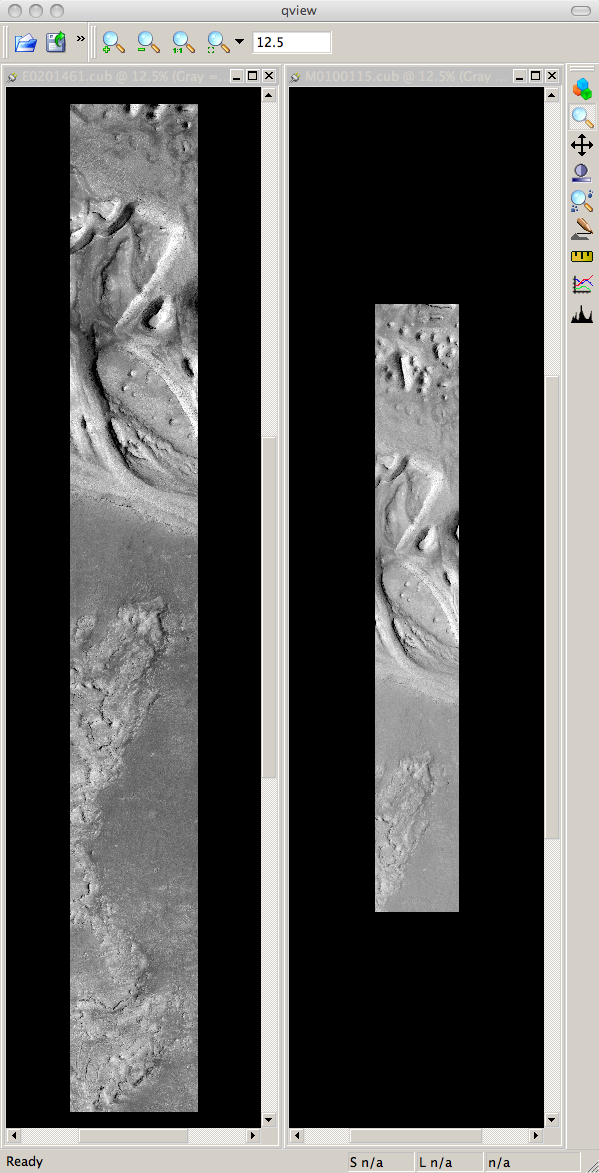
\includegraphics[height=3.7in]{images/p19-images.png}
\hfill
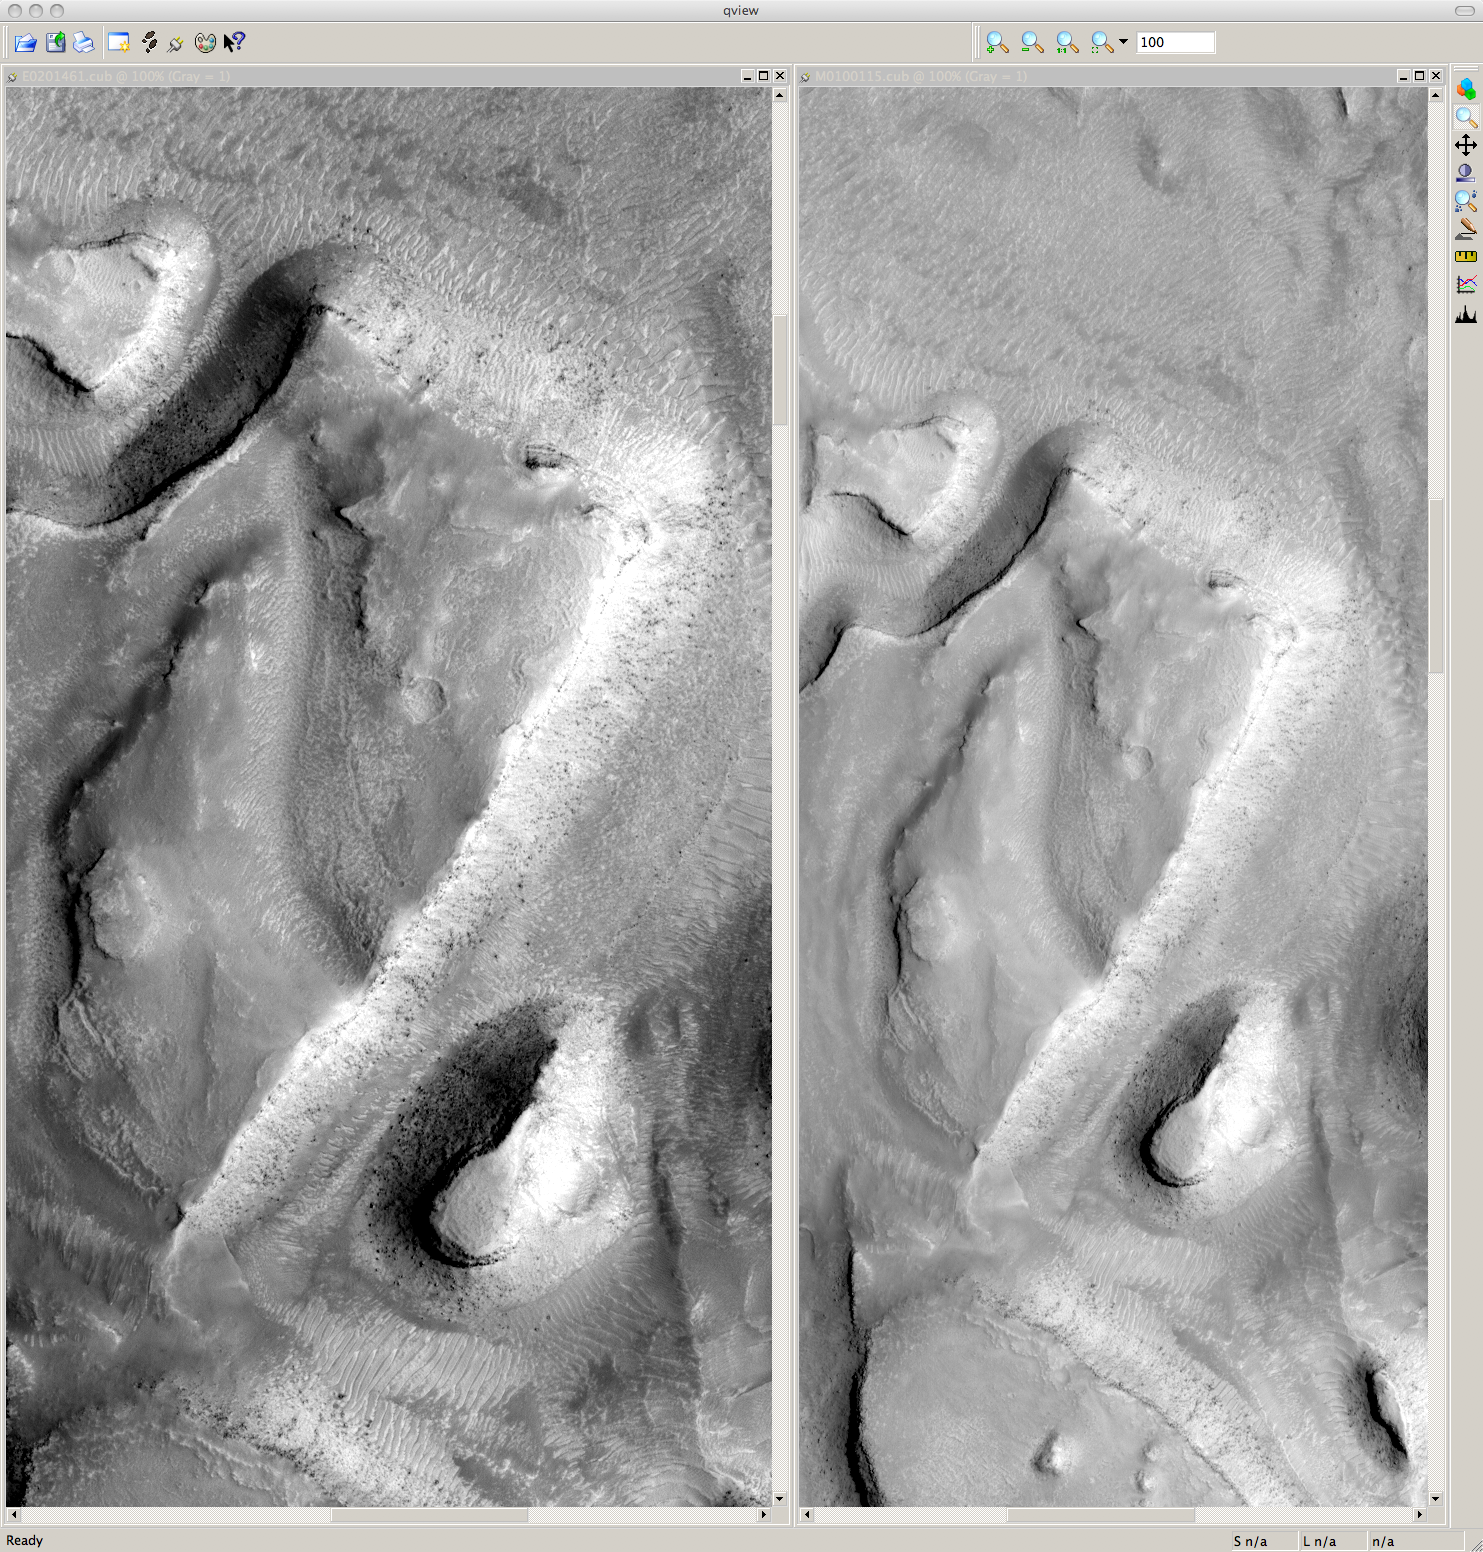
\includegraphics[height=3.7in]{images/p19-images_zoom.png}
\end{minipage}
\hfill
\begin{minipage}{1.3in}
\caption[P19 images open in qview zoomed in]{
    \label{p19-images}
    This figure shows \texttt{E0201461.cub} and \texttt{M0100115.cub}
    open in ISIS's qview program.  The view on the left shows their
    full extents at the same zoom level, showing how they have
    different ground scales.  The view on the right shows both images
    zoomed in on the same feature.  }
\end{minipage}
\end{figure}

\subsection{Aligning Images}
\label{sec:AligningImages}

The images also need to be rectified (or aligned).  There are many
ways to do this (for example, by setting \texttt{alignment-method} in \texttt{stereo}'s
\texttt{stereo.default} file, as described in section
\ref{settingoptionsinstereodefault}).  The most straightforward
process is to align the images by map-projecting them in \ac{ISIS}.
This example continues with the files from above, \texttt{E0201461.cub}
and \texttt{M010015.cub}.

This section describes the theory behind doing each of these steps,
but we also provide the \texttt{cam2map4stereo.py} program (page
\pageref{cam2map4stereo}) which performs these steps automatically
for you.

The \ac{ISIS} \texttt{cam2map} program will map-project these images:

\begin{verbatim}
  ISIS 3> cam2map from=M0100115.cub to=M0100115.map.cub
  ISIS 3> cam2map from=E0201461.cub to=E0201461.map.cub map=M0100115.map.cub matchmap=true
\end{verbatim}

Notice the order in which the images were run through
\texttt{cam2map}. The first projection with \texttt{M0100115.cub}
produced a map-projected image centered on the center of that image.
The projection of \texttt{E0201461.cub} used the \texttt{map=}
parameter to indicate that \texttt{cam2map} should use the same map
projection parameters as those of \texttt{M0100115.map.cub} (including
center of projection, map extents, map scale, etc.) in creating the
projected image. By map-projecting the image with the worse resolution
first, and then matching to that, we ensure two things: (1) that the
second image is summed or scaled down instead of being magnified up,
and (2) that we are minimizing the file sizes to make processing in
the Stereo Pipeline more efficient.

Technically, the same end result could be achieved by using the
\texttt{mocproc} program alone, and using its \texttt{map=
M0100115.map.cub} option for the run of \texttt{mocproc} on
\texttt{E0201461.cub} (it behaves identically to \texttt{cam2map}).
However, this would not allow for determining which of the two
images had the worse resolution and extracting their minimum
intersecting bounding box (see below).  Furthermore, if you choose
to conduct bundle adjustment (see Chapter \ref{ch:bundle_adjustment},
page \pageref{ch:bundle_adjustment}) as a pre-processing step, you
would do so between \texttt{mocproc} (as run above) and \texttt{cam2map}.

The above procedure is in the case of two images which cover similar
real estate on the ground.  If you have a pair of images where one
image has a footprint on the ground that is much larger than the
other, only the area that is common to both (the intersection of their
areas) should be kept to perform correlation (since non-overlapping
regions don't contribute to the stereo solution).  If the image with
the larger footprint size also happens to be the image with the better
resolution (i.e. the image run through \texttt{cam2map} second with
the \texttt{map=} parameter), then the above \texttt{cam2map}
procedure with \texttt{matchmap=true} will take care of it just fine.
Otherwise you'll need to figure out the latitude and longitude
boundaries of the intersection boundary (with the \ac{ISIS}
\texttt{camrange} program).  Then use that smaller boundary as the
arguments to the \texttt{MINLAT}, \texttt{MAXLAT}, \texttt{MINLON},
and \texttt{MAXLON} parameters of the first run of \texttt{cam2map}.
So in the above example, after \texttt{mocproc} with \texttt{Mapping=
  NO} you'd do this:

\begin{verbatim}[commandchars=\\\{\}]
  ISIS 3> camrange from=M0100115.cub
          \textnormal{[ ... lots of} camrange \textnormal{ output omitted ... ]}
  Group = UniversalGroundRange
    LatitudeType       = Planetocentric
    LongitudeDirection = PositiveEast
    LongitudeDomain    = 360
    MinimumLatitude    = 34.079818835324
    MaximumLatitude    = 34.436797628116
    MinimumLongitude   = 141.50666207418
    MaximumLongitude   = 141.62534719278
  End_Group
          \textnormal{[ ... more output of} camrange \textnormal{ omitted ... ]}
\end{verbatim}

\begin{verbatim}[commandchars=\\\{\}]
  ISIS 3> camrange from=E0201461.cub
          \textnormal{[ ... lots of} camrange \textnormal{ output omitted ... ]}
  Group = UniversalGroundRange
    LatitudeType       = Planetocentric
    LongitudeDirection = PositiveEast
    LongitudeDomain    = 360
    MinimumLatitude    = 34.103893080982
    MaximumLatitude    = 34.547719435156
    MinimumLongitude   = 141.48853937384
    MaximumLongitude   = 141.62919740048
  End_Group
          \textnormal{[ ... more output of} camrange \textnormal{ omitted ... ]}
\end{verbatim}

Now compare the boundaries of the two above and determine the intersection to use as the boundaries for \texttt{cam2map}:

\begin{verbatim}
  ISIS 3> cam2map from=M0100115.cub to=M0100115.map.cub DEFAULTRANGE=CAMERA \
                  MINLAT=34.10 MAXLAT=34.44 MINLON=141.50 MAXLON=141.63
  ISIS 3> cam2map from=E0201461.cub to=E0201461.map.cub map=M0100115.map.cub matchmap=true
\end{verbatim}

You only have to do the boundaries explicitly for the first run of
\texttt{cam2map}, because the second one uses the \texttt{map=}
parameter to mimic the map-projection of the first.  These two
images aren't radically different in areal coverage, so this isn't
really necessary for these images, its just an example.

Again, unless you are doing something complicated, using the
\texttt{cam2map4stereo.py} program (page \pageref{cam2map4stereo})
will take care of all these steps for you.

\section{Running the Stereo Pipeline}
\label{running-stereo}

Once the data has been prepared for processing, we invoke the 
\texttt{stereo} program (page \pageref{stereo}).

\subsection{Setting Options in the \texttt{stereo.default} File}
\label{settingoptionsinstereodefault}

The \texttt{stereo} program requires a \texttt{stereo.default} file that
contains settings that affect the stereo reconstruction process.  Its
contents can be altered for your needs; details are found in appendix
\ref{ch:stereodefault} on page \pageref{ch:stereodefault}.  You may find
it useful to save multiple versions of the \texttt{stereo.default} file
for various processing needs. If you do this, be sure to specify the desired
settings file by invoking \texttt{stereo} with the \texttt{-s}
option.  If this option is not given, the \texttt{stereo} program will
search for a file named \texttt{stereo.default} in the current working
directory. If \texttt{stereo} does not find \texttt{stereo.default} in
the current working directory and no file was given with the \texttt{-s}
option, \texttt{stereo} will assume default settings and continue.

The \texttt{stereo.default} example file distributed in the
\texttt{examples/} directory of \ac{ASP} has everything you need to process this
stereo pair. The actual file has a lot of comments to show you what
options and values are possible. Here's a trimmed version of the
important values in that file.
\begin{verbatim}
        alignment-method none
        cost-mode 2
        corr-kernel 21 21
        subpixel-mode 1
        subpixel-kernel 21 21
\end{verbatim}

\subsubsection*{Alignment Method}

The most important line in \texttt{stereo.default} is the
first one, specifying the alignment method. For raw images, alignment is
always necessary, as the left and right images are from different
perspectives. Several alignment methods are supported, including
\texttt{affineepipolar} and \texttt{homography} (see section 
\ref{stereo-default-preprocessing} for details). 

In this particular example, we will perform stereo with map-projected
images, in effect we take a smooth low-resolution terrain and map both
the left and right raw images onto that terrain. This automatically
brings both images in the same perspective, and as such, for
map-projected images the alignment method is always set to
\texttt{none}.

\subsubsection*{Correlation Parameters}

The second and third lines in \texttt{stereo.default} define what
correlation metric \textit{(normalized cross correlation)} we'll be
using and how big the template or kernel size should be \textit{(21
pixels square)}. A pixel in the left image will be matched to a pixel in
the right image by comparing the windows of this size centered at them.


\subsubsection*{Subpixel Refinement Parameters}

A highly critical parameter in \ac{ASP} is the value of
\texttt{subpixel-mode}, on the fourth line. When set to 1,
\texttt{stereo} performs parabola subpixel refinement, which is very
fast but not very accurate. When set to 2, it produces very accurate
results, but it is about an order of magnitude slower.

The fifth line sets the kernel size to use during subpixel refinement
\textit{(also 21 pixels square)}.

\subsubsection*{Search Range Determination}

Using these settings alone, \ac{ASP} will attempt to work out the
minimum and maximum disparity it will search for automatically. However if you
wish to, you can explicitly set the extent of the search range by
adding the option:
\begin{verbatim}
        corr-search -80 -2 20 2
\end{verbatim}

The exact values to use with this option you'll have to discover
yourself. The numbers right of the \texttt{corr-search} represents the
horizontal minimum boundary, vertical minimum boundary, horizontal
maximum boundary, and finally the horizontal maximum boundary.

Given that we map-projected the images using the same settings, you
may be wondering why there would still be an offset or search range at
all. The reason is twofold: (1) the camera position may be slightly
off, resulting in slight mis-alignment between stereo images; and then (2)
\ac{ISIS} doesn't have a perfect surface to project onto during map-projection, so small terrain features still produce changes in
perspective.  (In fact, these are precisely the features we are hoping
to detect!)

Given the uncertainties due to (1) and (2) above, it can be tricky to
select a good search range for the \texttt{stereo.default} file.
That's why the best way is to let \texttt{stereo} perform an automated
guess for the search range search. If you find that you can do a
better estimate of the search range, take look at the intermediate
disparity images using the \texttt{disparitydebug} program to figure
out which search directions can be expanded or contracted. The output
images will clearly show good data or bad data depending on whether
the search range is correct.

The worst case scenario is to determine search range manually by
opening both images in \texttt{qview} and comparing the coordinates
of points that you can match visually. Subtract line,sample locations
in the first image from the coordinates of the same feature in the
second image, and this will yield offsets that can be used in the search
range.  Make several of these offset measurements and use them to
define a line,sample bounding box, then expand this by 50\% and use
it for \texttt{corr-search}.  This will produce good results in
most images.

Also, if you are using an alignment option, you'll instead want to
make those disparity measurements against the written L and R tiff
files instead of the original input files.

\subsection{Performing Stereo Correlation}\label{perform-stereo}

Here is how the \texttt{stereo} program is invoked:

\begin{verbatim}
  ISIS 3> stereo E0201461.map.cub M0100115.map.cub \
            -s stereo.default.example results/output
\end{verbatim}

\noindent
That last option (\texttt{results/output}) is a prefix that
is used when generating names for \texttt{stereo} output files.  In
this case the first part is \texttt{results/}, which causes the
program to generate results in that directory with filenames that start
with \texttt{output}. If instead that last text was just
\texttt{output}, it would have created a collection of files
that start with \texttt{output} in the {\em same} directory as
the input files.

When \texttt{stereo} finishes, it will have produced a point cloud
image. Section \ref{visualising} describes how to convert it to a
digital elevation model (DEM) or other formats.

\subsection{Specifying Settings on the Command Line}

All the settings given via the \texttt{stereo.default} file can be
over-ridden from the command line. Just add a double hyphen
(\texttt{-\/-}) in front the option's name and then fill out the option
just as you would in the configuration file. For options in the
\texttt{stereo.default} file that take multiple numbers, they must be
separated by spaces (like `\texttt{corr-kernel~25~25}') on the command
line. Here is an example in which we override the search range and
subpixel mode from the command line.

\begin{verbatim}
  ISIS 3> stereo E0201461.map.cub M0100115.map.cub  \
            -s stereo.map --corr-search -70 -4 40 4 \
            --subpixel-mode 0 results/output
\end{verbatim}

\subsection{Stereo on Multiple Machines}

If the input images are really large, it may desirable to distribute the
work over several computing nodes. ASP provides a tool named
\texttt{parallel\_stereo} for that purpose. Its usage is described in section
\ref{parallel}.

\subsection{Diagnosing Problems}

Once invoked, \texttt{stereo} proceeds through several stages that are
detailed on page \pageref{entrypoints}.  Intermediate and final output
files are generated as it goes.  See Appendix
\ref{chapter:outputfiles}, page \pageref{chapter:outputfiles} for a
comprehensive listing.  Many of these files are useful for diagnosing and
debugging problems.  For example, as Figure~\ref{p19-stereo-output}
shows, a quick look at some of the TIFF files in the \texttt{results/}
directory provides some insight into the process.

\begin{figure}[t!]
\begin{minipage}{4in}
\includegraphics[width=4in]{images/p19-stereo-output.png}
\end{minipage}
\hfill
\begin{minipage}{2.9in}
\caption[P19 stereo output images]{
    \label{p19-stereo-output}
        These are the four viewable \texttt{.tif} files created by the
        \texttt{stereo} program.  On the left are the two aligned,
        pre-processed images: (\texttt{results/output-L.tif} and
        \texttt{results/output-R.tif}).  The next two are mask images
        (\texttt{results/output-lMask.tif} and
        \texttt{results/output-rMask.tif}), which indicate which
        pixels in the aligned images are good to use in stereo
        correlation.  The image on the right is the ``Good Pixel
        map'', (\texttt{results/output-GoodPixelMap.tif}), which
        indicates (in gray) which were successfully matched with the
        correlator, and (in red) those that were not matched.}
\end{minipage}
\end{figure}

Perhaps the most accessible file for assessing the quality of your
results is the good pixel image,
\\ (\texttt{results/output-GoodPixelMap.tif}).  If this file shows
mostly good, gray pixels in the overlap area (the area that is white
in both the \texttt{results/output-lMask.tif} and
\texttt{results/output-rMask.tif} files), then your results are
just fine.  If the good pixel image shows lots of failed data,
signified by red pixels in the overlap area, then you need to go back
and tune your \texttt{stereo.default} file until your results improve.
This might be a good time to make a copy of \texttt{stereo.default} as
you tune the parameters to improve the results.

You should also know that whenever the \texttt{stereo} executable is
run, it makes a copy of the configuration file used in
\textit{output-prefix}-stereo.default. Opening that output file will
show when the command was run, what the flags were from the command
line, and then a copy of the \texttt{stereo.default}. This will
hopefully help debug and log what was performed so that others in the
future can recreate your work.

Another handy debugging tool is the \texttt{disparitydebug} program,
which allows you to generate viewable versions of the intermediate
results from the stereo correlation algorithm.
\texttt{disparitydebug} converts information in the disparity image
files into two TIFF images that contain horizontal and vertical
components of the disparity (i.e. matching offsets for each pixel in
the horizontal and vertical directions).  There are actually three
flavors of disparity map: the \texttt{-D.tif}, the \texttt{-RD.tif},
and \texttt{-F.tif}.  You can run \texttt{disparitydebug} on any of
them.  Each shows the disparity map at the different stages of
processing.

\begin{verbatim}
  >  disparitydebug results/output-F.tif
\end{verbatim}

If the output H and V files from \texttt{disparitydebug} look good,
then the point cloud image is most likely ready for post-processing.
You can proceed to make a mesh or a \ac{DEM} by processing
\texttt{results/output-PC.tif} using the \texttt{point2mesh} or
\texttt{point2dem} tools, respectively.

Figure \ref {p19-disparity} shows the outputs of \texttt{disparitydebug}.

\begin{figure}[b!]
\begin{minipage}{4in}
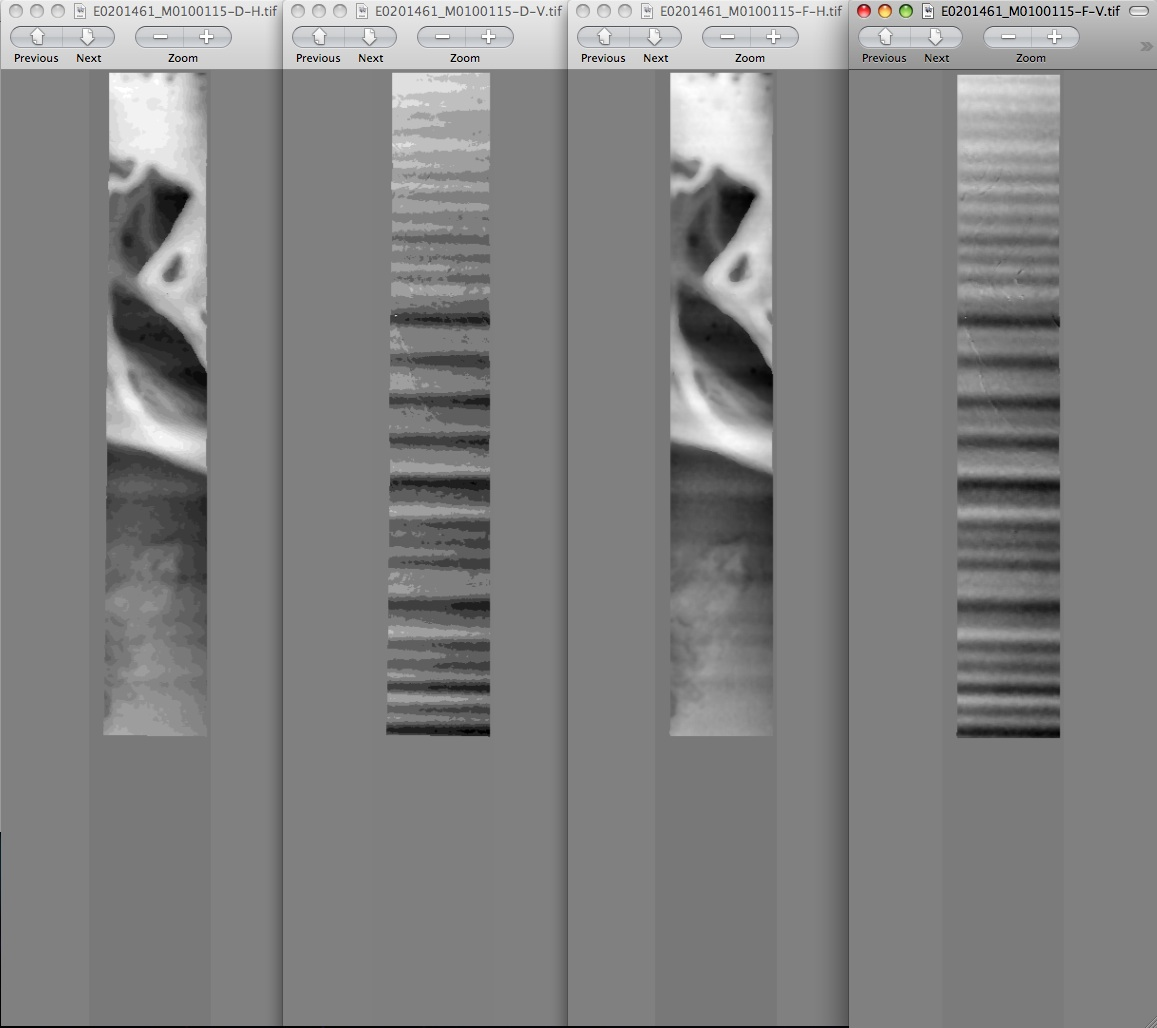
\includegraphics[width=4in]{images/p19-disparity.png}
\end{minipage}
\hfill
\begin{minipage}{2.7in}
\caption[P19 disparity images]{
    \label{p19-disparity}
	Disparity images produced using the \texttt{disparitydebug}
        tool.  The two images on the left are the
        \texttt{results/output-D-H.tif} and
        \texttt{results/output-D-V.tif} files, which are normalized
        horizontal and vertical disparity components produced by the
        disparity map initialization phase.  The two images on the
        right are \texttt{results/output-F-H.tif} and
        \texttt{results/output-F-V.tif}, which are the final
        filtered, sub-pixel-refined disparity maps that are fed into the
        Triangulation phase to build the point cloud image.  Since
        these MOC images were acquired by rolling the spacecraft
        across-track, most of the disparity that represents topography
        is present in the horizontal disparity map.  The vertical
        disparity map shows disparity due to ``wash-boarding,'' which
        is not from topography but from spacecraft movement. Note
        however that the horizontal and vertical disparity images are
        normalized independently.  Although both have the same range
        of gray values from white to black, they represent
        significantly different absolute ranges of disparity.}
\end{minipage}
\end{figure}

\section{Visualizing and Manipulating the Results}
\label{visualising}

When \texttt{stereo} finishes, it will have produced a point cloud
image.  At this point, many kinds of data products can be built from
the \texttt{results/output-PC.tif} point cloud file.

\subsection{Building a 3D Model}

If you wish to see the data in an interactive 3D browser, then you can
generate a 3D object file using the \texttt{point2mesh} command (page
\pageref{point2mesh}). The resulting file is stored in Open Scene
Graph binary format \cite{OSG_website}.  It can be viewed with
\texttt{osgviewer} (the Open Scene Graph Viewer program, distributed
with the binary version of the Stereo Pipeline).  The
\texttt{point2mesh} program takes the point cloud file and the left
normalized image as inputs:

\begin{verbatim}
  > point2mesh results/output-PC.tif results/output-L.tif -l
  > osgviewer results/output.ive
\end{verbatim}

The image displayed by \texttt{osgviewer} is shown in figure \ref{p19-osg}.

When the \texttt{osgviewer} program starts, you may want to toggle the
lighting with the `L' key, toggle texturing with the 'T' key, and
toggle wireframe mode with the 'W'.  Press '?' to see a variety of
other interactive options. 

\begin{figure}[h!]
\begin{minipage}{5in}
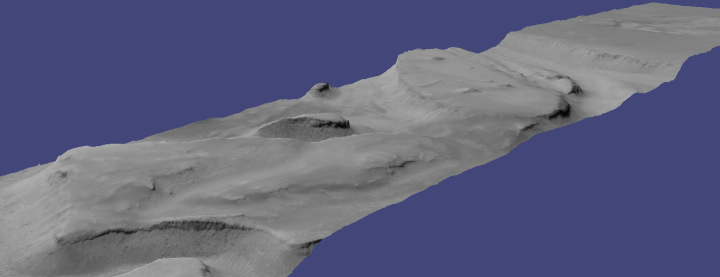
\includegraphics[width=5in]{images/p19-osg.png}
\end{minipage}
\hfill
\begin{minipage}{1.7in}
\caption[P19 in OSG]{
    \label{p19-osg}
	The \texttt{results/output.ive} file displayed in the OSG
        Viewer.}
\end{minipage}
\end{figure}

\subsection{Building a Digital Elevation Model}

The \texttt{point2dem} program (page \pageref{point2dem}) creates a
Digital Elevation Model (\ac{DEM}) from the point cloud file.

\begin{verbatim}
  >  point2dem results/output-PC.tif
\end{verbatim}

\noindent
The resulting TIFF file is map-projected and will contain
georeferencing information stored as GeoTIFF tags. You can specify a
coordinate system (e.g., mercator, sinusoidal) and a reference
spheroid (i.e., calculated for the Moon, Mars, or Earth).

\begin{verbatim}
  >  point2dem -r mars results/output-PC.tif
\end{verbatim}

\noindent
This product is suitable for scientific use, and can be imported into
a variety of GIS platforms.  However, the resulting file,
\texttt{results/output-DEM.tif}, will have 32-bit floating point
pixels, and will not render well in typical image viewers.

The \texttt{point2dem} program can also be used to orthoproject raw
satellite imagery onto the \ac{DEM}. To do this, invoke
\texttt{point2dem} just as before, but add the \texttt{-\/-orthoimage}
option and specify the use of the left image file as the texture file
to use for the projection:

\begin{verbatim}
  >  point2dem -r mars --orthoimage results/output-L.tif \
       results/output-PC.tif
\end{verbatim}

See figure \ref{p19-norm_ortho} on the right for the output of this command.

\noindent
The \texttt{point2dem} program is also able to accept output
projection options the same way as the tools in GDAL. Well known EPSG,
IAU2000 projections, and custom Proj4 strings can applied with the
target spatial reference set flag, \texttt{-\/-t\_srs}. If the target
spatial reference flag is applied with any of the reference spheroid
options, the reference spheroid option will overwrite the datum
defined in the target spatial reference set. The following examples
produce the same output.

\begin {verbatim}
  >  point2dem --t_srs IAU2000:49900 results/output-PC.tif
  >  point2dem --t_srs "+proj=longlat +a=3396190 +b=3376200"
       results/output-PC.tif
\end{verbatim}

\noindent
The \texttt{point2dem} program can be used in many different ways.  Be
sure to take your time to explore all of the options.

\begin{figure}
\hfill
\begin{minipage}{3.5in}
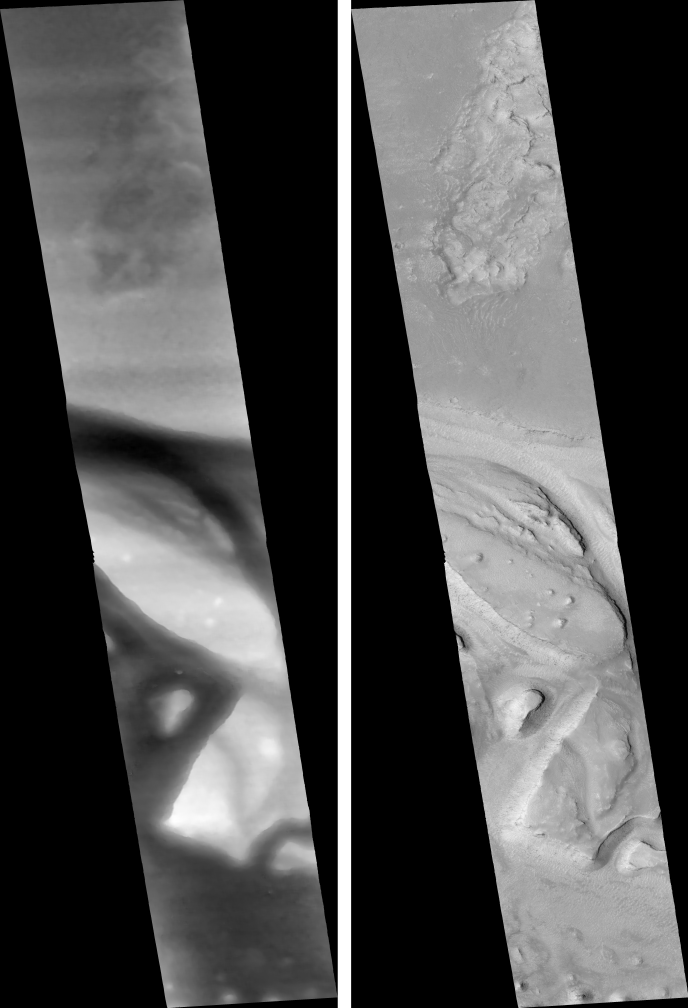
\includegraphics[width=3.5in]{images/p19-norm_ortho.png}
\end{minipage}
\hfill
\begin{minipage}{2in}
\caption[P19 Normalized DEM and Orthophoto]{
    \label{p19-norm_ortho}
	The image on the left is a normalized DEM (generated using
        \texttt{point2dem}'s 
        \texttt{-n} option), which shows low terrain values as black
        and high terrain values as white.  The image on the right is
        the left input image projected onto the DEM (created using the
        \texttt{-\/-orthoimage} option to \texttt{point2dem}).  }
\end{minipage}
\hfill
\end{figure}

% \begin{figure}
% \begin{center}
% 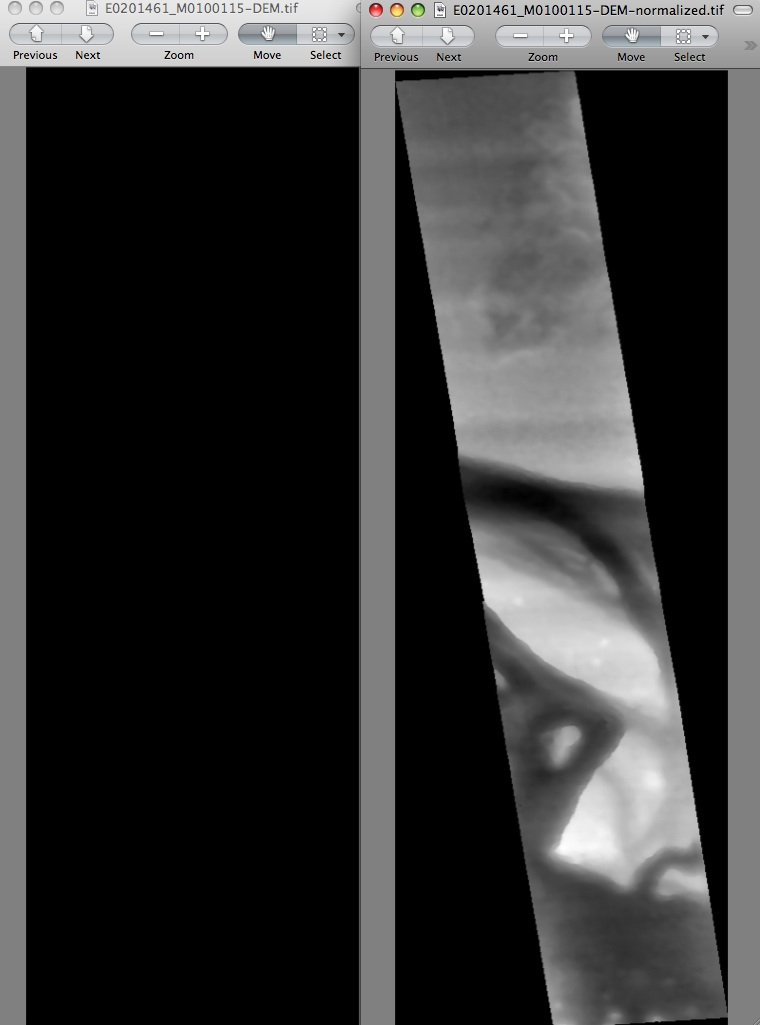
\includegraphics[width=4in]{images/p19-dems.png}
% \caption[P19 dem images]{
%     \label{p19-dems}
%	The non-normalized and normalized DEMs. Note that the
%	non-normalized version contains floating point pixel values
%	and will not open in most image viewing programs which
%	expect integer pixel values between 0 and 255 (which is
%	what the normalized version does for you).
%     }
% \end{center}
% \end{figure}
%
% \begin{figure}
% \begin{center}
% \includegraphics[width=3in]{images/p19-ortho.png}
% \caption[P19 orthophoto]{
%     \label{p19-ortho}
%	The left image orthoprojected onto the DEM.
%     }
% \end{center}
% \end{figure}

\subsection{Alignment to point clouds from a different source}

Often times, the 3D terrain models output by \texttt{stereo} (point
clouds and DEMs) can be intrinsically quite accurate, yet their actual
position on the planet may be off by up to several tens of meters. This
can result from small errors in the position and orientation of the
satellite cameras taking the pictures.

ASP provides a tool named \texttt{pc\_align} for aligning such 3D
terrains to a much more accurately positioned (if potentially sparser)
dataset. Such datasets can be made up of ground control points (in the
case of Earth), or from laser altimetry instruments on satellites, such
as ICESat/GLASS for Earth, LRO/LOLA on the Moon, and MGS/MOLA on Mars.

Under the hood, \texttt{pc\_align} uses Iterative Closest Point (ICP),
which works best when the point cloud held fixed in place as reference
is denser than the one being transformed to align to it, which is the
opposite of what we would need in our case, as we'd like to move the
dense output of \texttt{stereo} to align to the accurately known sparser
dataset. Yet this is not a problem since we can use ICP as it works
best, and then simply invert the alignment transform and apply it to the
ASP point cloud so that it aligns to the accurately positioned dataset.

The \texttt{pc\_align} tool requires another input, an apriori guess for
the maximum displacement we expect to see as result of alignment, that
is, by how much the points will move when the alignment transform is
applied. If not known, a large (but not unreasonably so) number can be
specified. It is used to remove most of the points in the source
(moveable) point cloud which have no chance of having a corresponding
point in the reference (fixed) point cloud.

Here is how \texttt{pc\_align} can be called.

\begin {verbatim}
  >  pc_align --max-displacement 200 --datum D_MARS \
       --save-inv-transformed-reference-points      \
       results/output-PC.tif mola.csv
\end{verbatim}

The complete documentation for this program is in section
\ref{pcalign}.

\subsection{Creating DEMs relative to the Geoid/Areoid}

The DEMs generated using \texttt{point2dem} are in reference to a datum
ellipsoid. If desired, the \texttt{dem\_geoid} program can be used to
convert this DEM to be relative to a geoid/areoid on Earth/Mars
respectively.

\begin {verbatim}
  >  dem_geoid results/output-DEM.tif 
\end{verbatim}

\subsection{Converting to the LAS Format}

If it is desired to use the generated point cloud in contexts outside
ASP, it can be converted to the LAS file format, which is a public file
format for the interchange of 3-dimensional point cloud data. The tool
\texttt{point2las} can be used for that purpose (section \ref{point2las}).

\begin {verbatim}
  >  point2las --compressed results/output-PC.tif 
\end{verbatim}

\subsection{Generating Color Hillshade Maps}

Once you have generated a \ac{DEM} file, you can use the Vision Workbench's
\texttt{colormap} and \texttt{hillshade} tools to create colorized
and/or shaded relief images.

To create a colorized version of the \ac{DEM}, you need only specify
the \ac{DEM} file to use. The colormap is applied to the full range of
the DEM, which is computed automatically.  Alternatively you can
specific your own min and max range for the color map.

\begin{verbatim}
  >  colormap results/output-DEM.tif -o hrad-colorized.tif
\end{verbatim}

To create a hillshade of the \ac{DEM}, specify the \ac{DEM} file to
use. You can control the azimuth and elevation of the light source
using the \texttt{-a} and \texttt{-e} options.

\begin{verbatim}
  >  hillshade results/output-DEM.tif -o hrad-shaded.tif -e 25
\end{verbatim}

To create a colorized version of the shaded relief file, specify
the \ac{DEM} and the shaded relief file that should be used:

\begin{verbatim}
  >  colormap results/output-DEM.tif -s hrad-shaded.tif -o hrad-color-shaded.tif
\end{verbatim}

See figure \ref{hrad-color} showing the images obtained with these commands.

\begin{figure}[b!]
\begin{center}
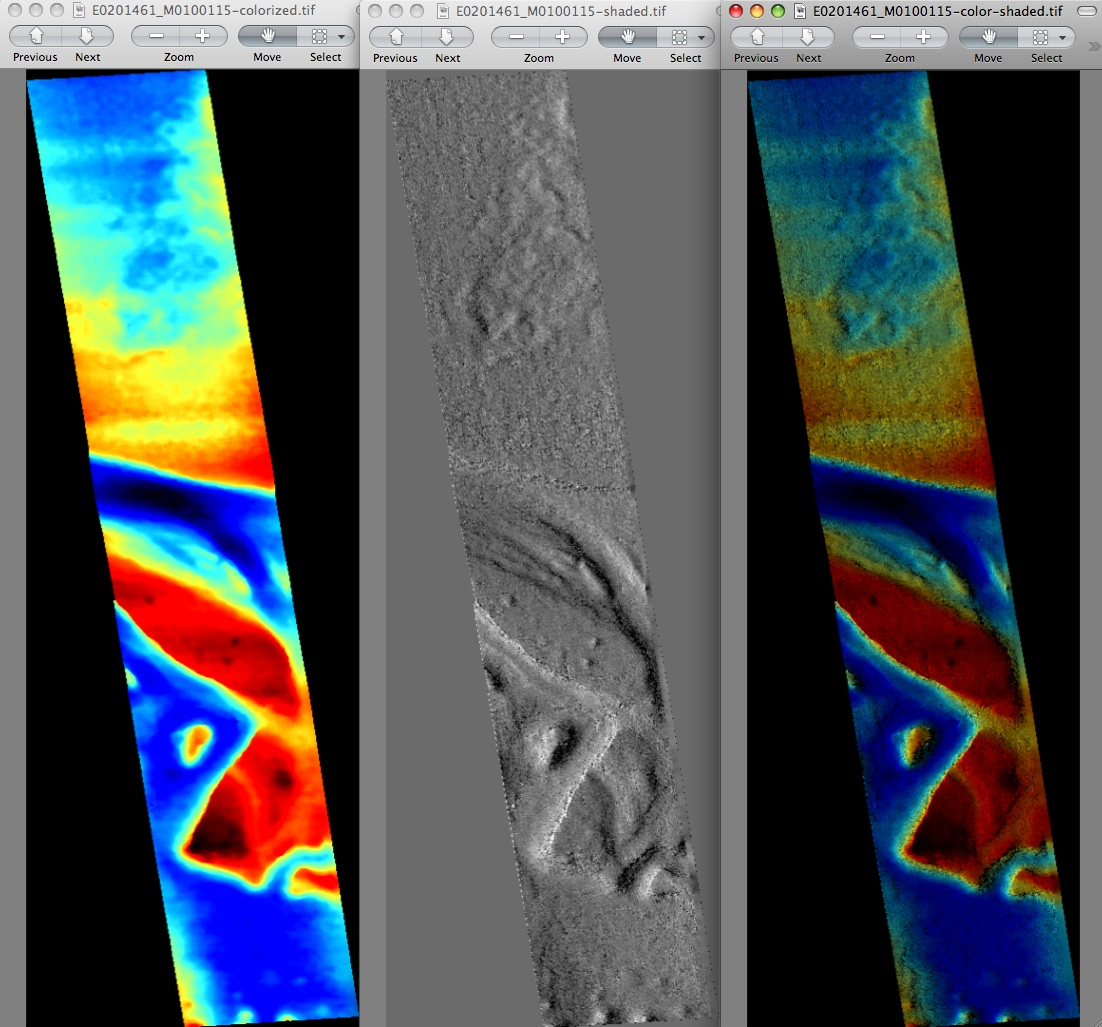
\includegraphics[width=4.7in]{images/p19-colorized-shaded.png}
\caption[Hrad colorized and shaded relief]{
    \label{hrad-color}
	The colorized DEM, the shaded relief image, and the colorized hillshade.
    }
\end{center}
\end{figure}

\subsection{Building Overlays for Moon and Mars mode in Google Earth}

The final program in the Stereo Pipeline package that this tutorial
will address is \texttt{image2qtree}.  This tool was designed to
create tiled, multi-resolution overlays for Google Earth.  In addition
to generating image tiles, it produces a metadata tree in KML format
that can be loaded from your local hard drive or streamed from a
remote server over the Internet.

The \texttt{image2qtree} program can only be used on 8-bit image files
with georeferencing information (e.g. grayscale or RGB geotiff
images). In this example, it can be used to process 

\texttt{results/output-DEM-normalized.tif}, \texttt{results/output-DRG.tif}, \texttt{hrad-shaded.tif}, \\
\texttt{hrad-colorized.tif}, and \texttt{hrad-shaded-colorized.tif}.

These images were generated respectively by using \texttt{point2dem}
with the \texttt{-n} option creating a normalized DEM, the
\texttt{-\/-orthoimage} option to \texttt{point2dem} which projects the
left image onto the DEM, and the images created earlier with
\texttt{colormap}.

\begin{verbatim}
  >  image2qtree hrad-shaded-colorized.tif -m kml --draw-order 100
\end{verbatim}

Figure \ref{hrad-kml} shows the obtained KML files in Google Earth.

\begin{figure}[b!]
\begin{center}
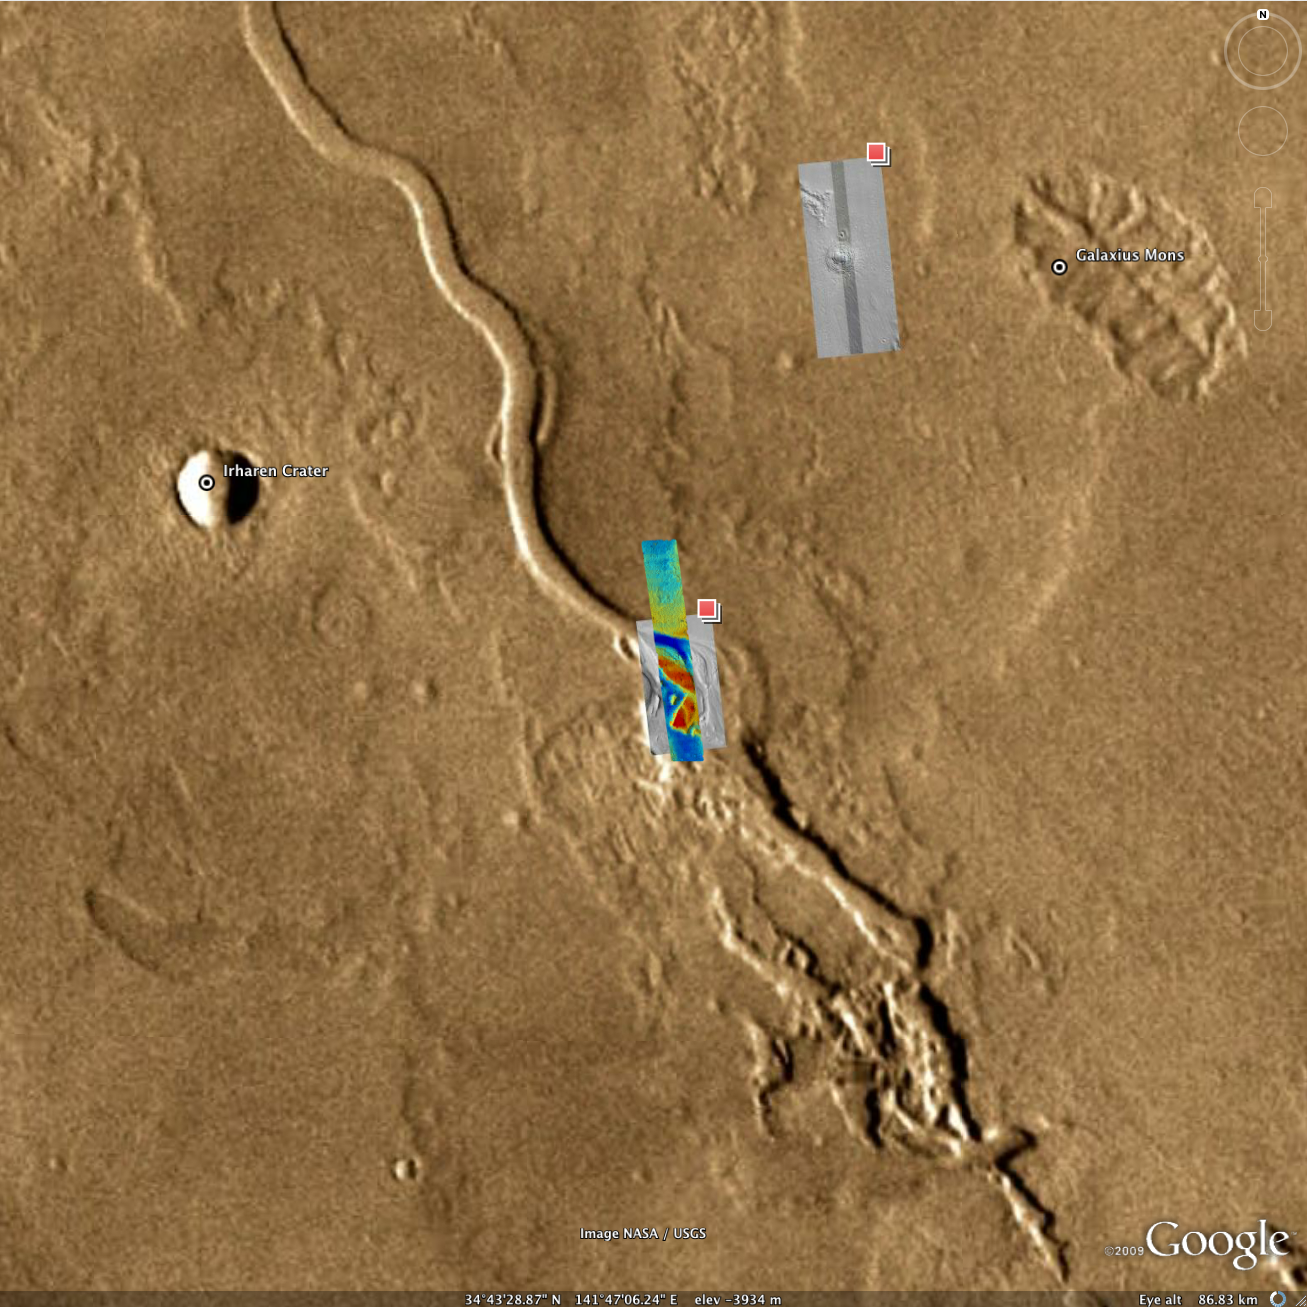
\includegraphics[width=6in]{images/p19-googlemars.png}
\caption[Hrad shaded colorized DEM as a KML overlay] {
    \label{hrad-kml}
        The colorized hillshade DEM as a KML overlay.  }
\end{center}
\end{figure}

\chapter{Tutorial: Processing Digital Globe Imagery}
\label{ch:dg_tutorial}

Digital Globe provides imagery from the Quick Bird and the three World
View satellites. These are the hardest images to process with Ames
Stereo Pipeline because they are exceedingly large, much larger than
HiRISE imagery. There is also a wide range of terrain challenges and
atmospheric effects that can confuse ASP. Trees are particularly
difficult for us since their texture is nearly nadir and perpendicular
to our line of sight. It is important to know that the driving force
behind our support for Digital Globe imagery is to create models of
ice and bare rock. That is the type of imagery that we have tested
with and have focused on. If we can make models of wooded or urban
areas, that is a bonus, but we can't provide any advice for how to
perform or improve the results if you choose to use ASP in that way.

ASP can only process Level 1B imagery and cannot process Digital Globe's
aerial imagery. We can pull a camera model from the RPC coefficients or
from their linear camera model described in the provided XML files. We
won't be discussing the RPC method in this section, however you can
learn more about it in the later example (section \ref{rpc}) where we
discuss processing GeoEye imagery which comes only with RPC
coefficients.

Our implementation of the linear camera model only
models the geometry of the imaging hardware itself and velocity
aberration. We do not currently model refraction due to light bending
in Earth's atmosphere. It is our understanding that this could
represent misplacement of points up to a meter for some
imagery. However this is still smaller error than the error from
measurement of the spacecraft's position and orientation. We do not
provide facilities for correcting spacecraft attitude either. So you
will have to perform some manual shifting of the data to get it into
the correct location. These errors are fortunately much less than
found with extra-terrestrial missions largely due to the availability
of GPS and high bandwidth comms with the satellite.

In the next 2 sections we will show how to process unmodified and
map-projected variants of World View 1 imagery. This steps will be the
same for Digital Globe's other satellites. The imagery we are using are
from the free stereo pair example of Lucknow, India available from
Digital Globe's website \cite{digital-globe:samples}. These images
represent a non-ideal problem for us since this is an urban location,
but at least you should be able to download this imagery yourself and
follow along.

\section{Processing Raw}
\label{rawdg}

After you have downloaded the example stereo imagery of India, you
will find a directory titled\newline
\texttt{052783824050\_01\_P001\_PAN}. It has a
lot of files and many of them contain redundant information just
displayed in different formats. We are interested only in the TIF or NTF
imagery and the similarly named XML file. 

Further investigation of the files downloaded will show that there are
in fact 4 image files. This is because Digital Globe breaks down a
single observation into multiple files for what we assume are size
reasons. These files have a pattern string of ``\_R[N]C1-'', where N
increments for every subframe of the full observation. The tool named
\texttt{dg\_mosaic} can be used to mosaic (and optionally reduce the
resolution of) such a set of sub-observations into a single image file
and create an appropriate camera file 

\begin{verbatim}
    > dg_mosaic 12FEB12053305*TIF --output-prefix 12FEB12053305 --reduce-percent 50
\end{verbatim}

and anologously for the second set. See section \ref{dgmosaic} for more
details. The \texttt{stereo} program can use either the original or the mosaicked images.

Since we are ingesting these images raw, it is strongly recommended that
you use an affine epipolar alignment to reduce the search range. The
\texttt{stereo} command and a rendering in QGIS are shown below.

\begin{verbatim}
    > stereo -t dg                                            \
             12FEB12053305-P1BS_R2C1-052783824050_01_P001.TIF \
             12FEB12053341-P1BS_R2C1-052783824050_01_P001.TIF \
             12FEB12053305-P1BS_R2C1-052783824050_01_P001.XML \
             12FEB12053341-P1BS_R2C1-052783824050_01_P001.XML dg/dg
\end{verbatim}

\begin{figure}[h!]
\centering
  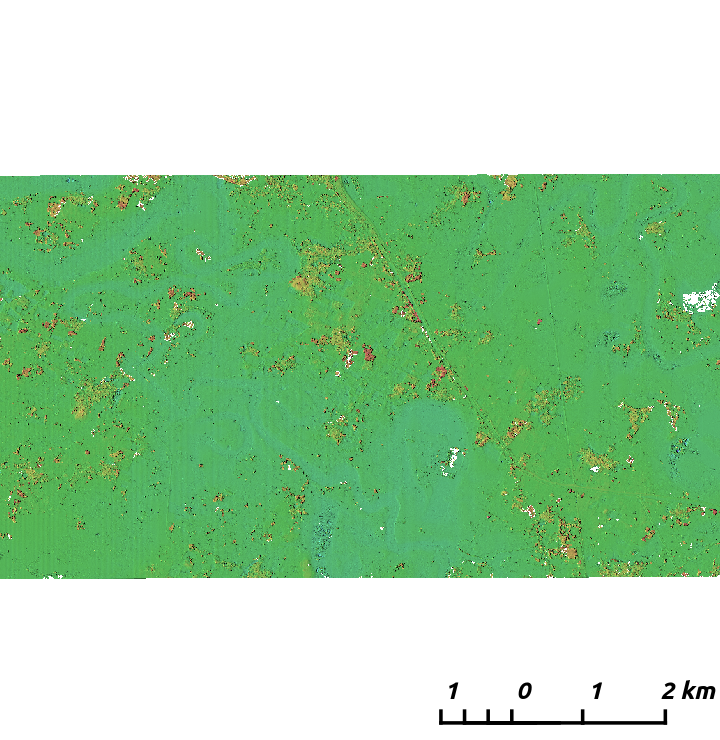
\includegraphics[width=2.0in]{images/examples/dg/DigitalGlobeContext.png}
  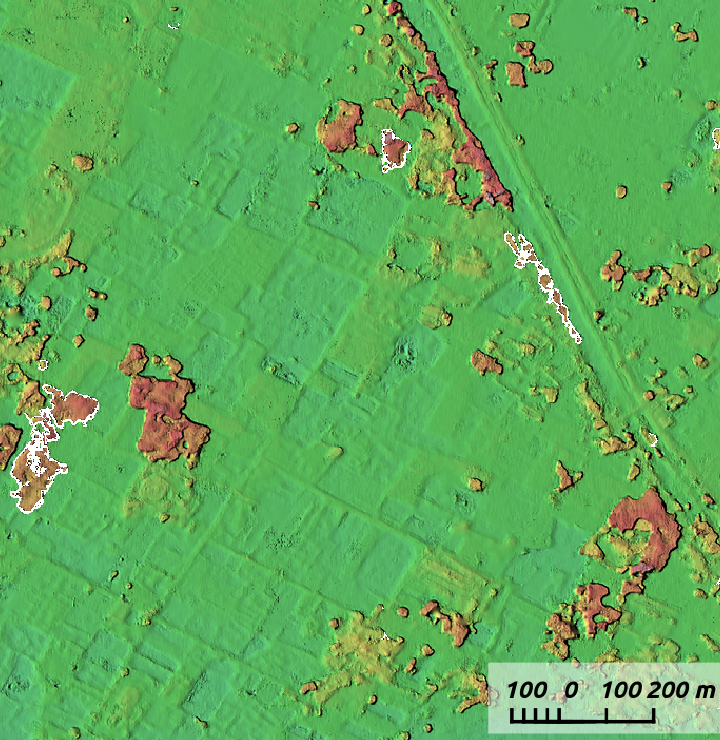
\includegraphics[width=2.0in]{images/examples/dg/DigitalGlobeCloseUp.png}
  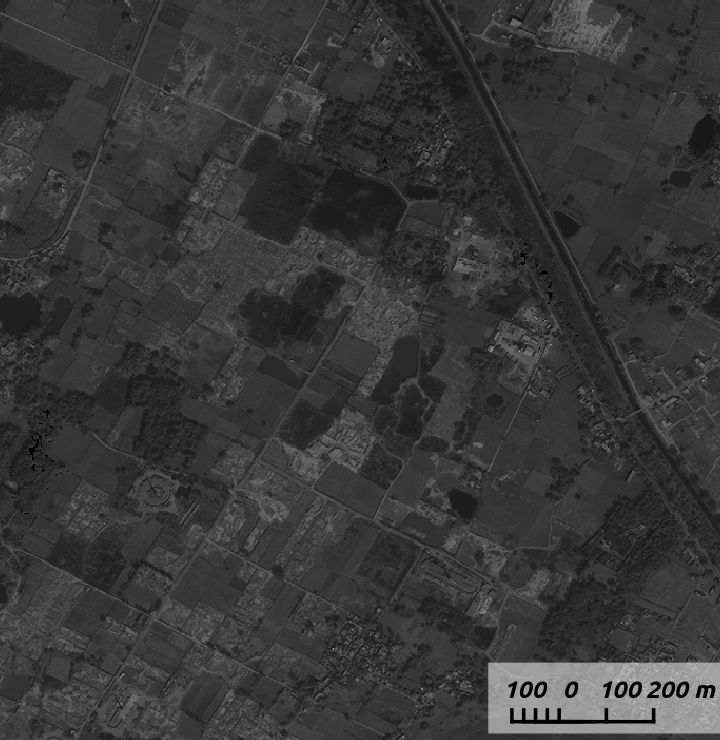
\includegraphics[width=2.0in]{images/examples/dg/DigitalGlobeCloseUpDRG.png}
\caption{Example colorized height map and ortho image output.}
\label{fig:dg-nomap-example}
\end{figure}

It is important to note that we could have performed stereo using the
approximate RPC model instead of the exact linear camera model (both
models are in the same XML file), by switching the session in the
\texttt{stereo} command above from \texttt{-t dg} to \texttt{-t
rpc}. The RPC model is somewhat less accurate, so the results will not
be the same, in our experiments we've seen differences in the 3D
terrains using the two approaches of 5 meters or more.

\subsubsection*{stereo.default}

The stereo.default example file (appendix \ref{ch:stereodefault}) works
generally well with all Digital Globe pairs. Just set
\texttt{alignment-method} to \texttt{affineepipolar} or
\texttt{homography}, since in this case we are using non-projected
images.

\section{Processing Map-Projected Imagery}
\label{mapproj}

Eventually you will run into Digital Globe imagery that has too much
parallax to be processed in a reasonable time. (That wasn't the case for
Lucknow, India because it is so flat.) We can speed up the result by
performing stereo on map-projected versions of the images. The
map-projection is done with a tool named \texttt{mapproject}. It uses
the simplified RPC model contained in the camera XML file to project a
given camera image onto a pre-determined low-resolution DEM without
holes.

ASP will then perform correlation on the map-projected images, and,
before doing triagulation will internally project back the image pixels
onto the original camera locations, precisely reversing the
transformation done with \texttt{mapproject}.

The hardest part of this whole process is getting the input
low-resolution DEM. In this example we will use a variant of NASA
SRTM data with no holes. Other choices might be GMTED2010 or USGS's NED
data.

It is important to note that ASP expects the input low-resolution DEM to
be in reference to a datum ellipsoid, such as WGS84 or NAD83. If the DEM
is in respect to either the EGM96 or NAVD88 geoids, the ASP tool
\texttt{dem\_geoid} can be used to convert the DEM to WGS84 or NAD83
(section \ref{demgeoid}). (The same tool can be used to convert back the
final output ASP DEM to be in reference to a geoid, if desired.)

Not applying this conversion might not properly negate the parallax
seen between the two images, though it will not corrupt the
triangulation results. In other words, sometimes one may get by
ignoring the vertical datums on the input but we do not recommend
doing that. Also, you should note that the geoheader attached to those
types of files usually do not describe the vertical datum they
used. That can only be understood by careful reading of your
provider's documents.

In this example we as input low-resolution DEM the file
\texttt{srtm\_53\_07.tif}, a 90 meter resolution tile from the CGIAR-CSI
modification of the original NASA SRTM product \cite{cgiar:srtm90m}.
The NASA SRTM square for this example spot in India is N26E080.

Below are the commands for map-projecting the input and then running
through stereo. You can use any projection you like as long as it
preserves detail in the imagery. Note that the last parameter in the
stereo call is the input low-resolution DEM.

\begin{figure}[h!]
\centering
  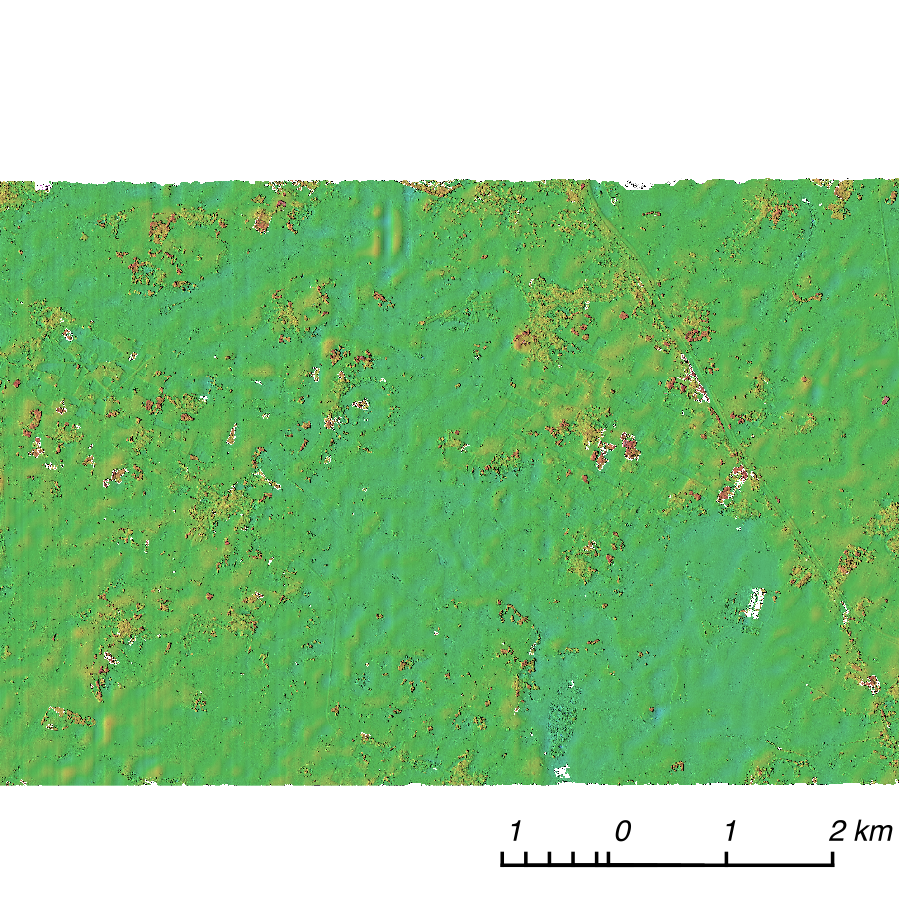
\includegraphics[width=2.0in]{images/examples/dg/MappedContext.png}
  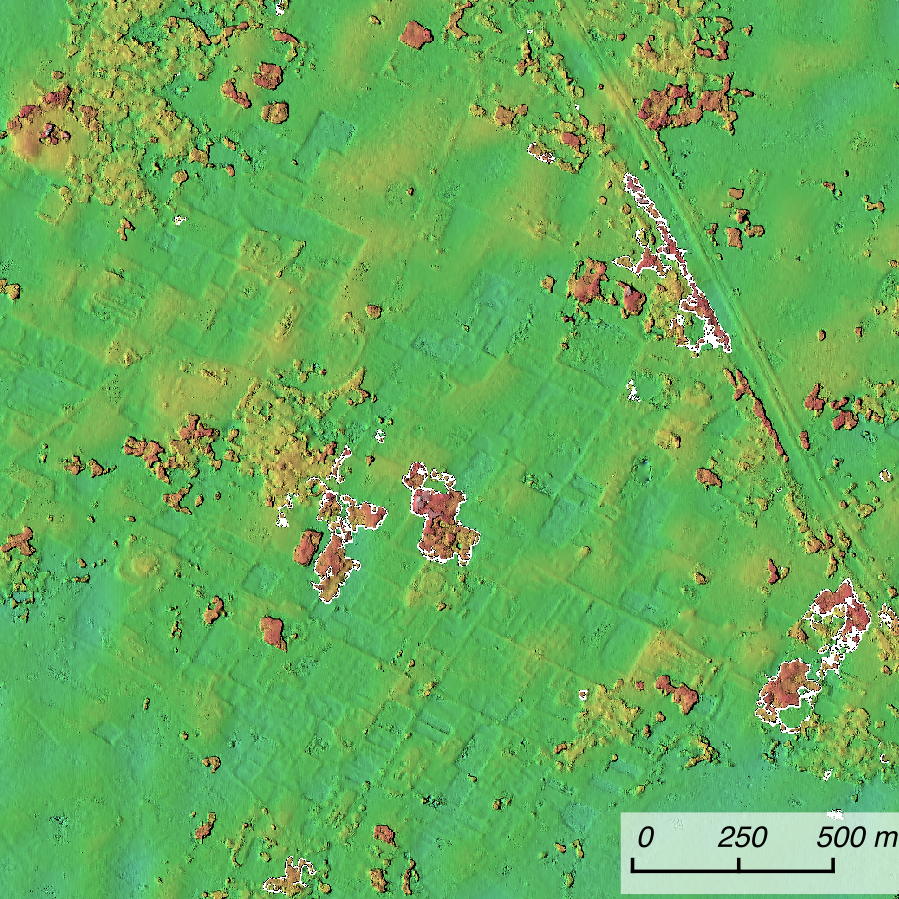
\includegraphics[width=2.0in]{images/examples/dg/MappedCloseUp.png}
  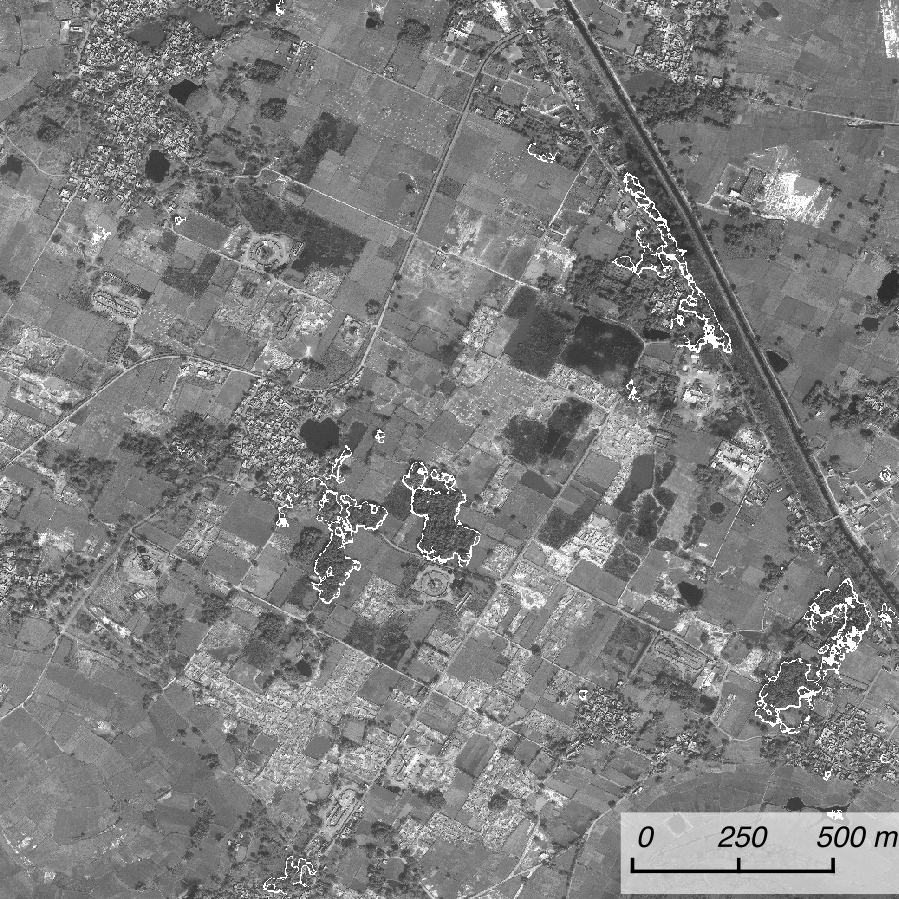
\includegraphics[width=2.0in]{images/examples/dg/MappedCloseUpDRG.png}
\caption{Example colorized height map and ortho image output.}
\label{fig:dg-map-example}
\end{figure}

\subsubsection*{Commands}

\begin{verbatim}
    > mapproject -t rpc --t_srs "+proj=eqc +units=m +datum=WGS84" \
        --tr 0.5 srtm_53_07.tif \
        12FEB12053305-P1BS_R2C1-052783824050_01_P001.TIF \
        12FEB12053305-P1BS_R2C1-052783824050_01_P001.XML \
        left_mapped.tif
    > mapproject -t rpc --t_srs "+proj=eqc +units=m +datum=WGS84" \
        --tr 0.5 srtm_53_07.tif \
        12FEB12053341-P1BS_R2C1-052783824050_01_P001.TIF \
        12FEB12053341-P1BS_R2C1-052783824050_01_P001.XML \
        right_mapped.tif
    > stereo -t dg left_mapped.tif right_mapped.tif           \
             12FEB12053305-P1BS_R2C1-052783824050_01_P001.XML \
             12FEB12053341-P1BS_R2C1-052783824050_01_P001.XML \
             dg/dg srtm_53_07.tif
\end{verbatim}

If the \texttt{--t\_srs} option is not specified, it will be read from
the low-resolution input DEM.

The complete list of options for \texttt{mapproject} is described in
section \ref{mapproject}.

\subsubsection*{stereo.default}

The stereo.default example file (appendix \ref{ch:stereodefault}) works
generally well with all Digital Globe pairs. Just set
\texttt{alignment-method} to \texttt{none} since the images are
map-projected.

\section{Handling CCD Boundary Artifacts}

\begin{figure}[h!]
\centering
  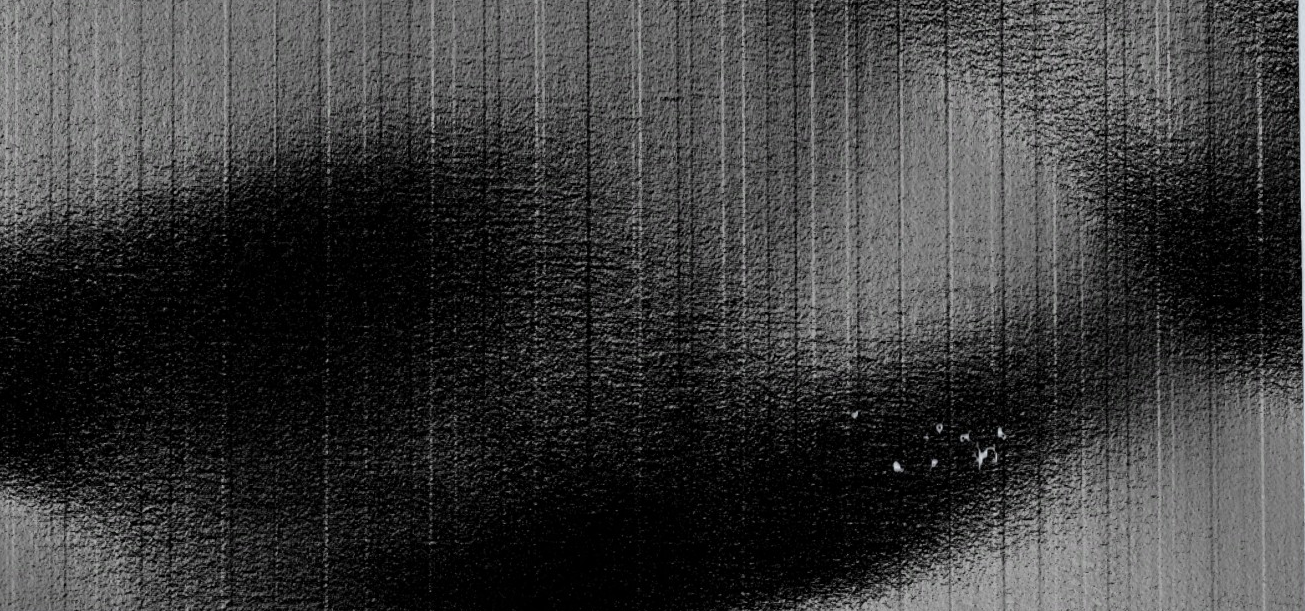
\includegraphics[width=3.0in]{images/examples/ccd_before.png}
  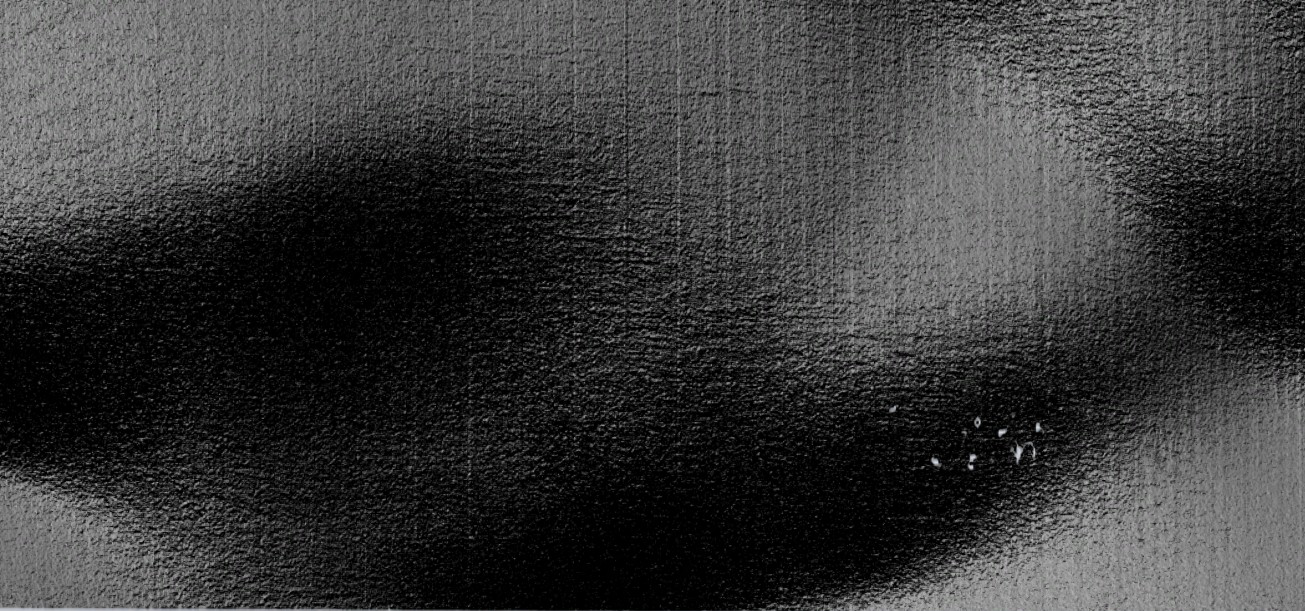
\includegraphics[width=3.0in]{images/examples/ccd_after.png}
\caption{Example of of a hillshaded terrain obtained using stereo without (left) and with (right) CCD boundary artifact correction applied using \texttt{wv\_correct}.}
\label{fig:ccd-artifact-example}
\end{figure}

An image taken by one of Digital Globe's World View satellite cameras is
formed of several blocks as tall as the image, mosaicked from left to
right, with each block coming from an individual CCD sensor
\cite{digital-globe:camera}. Particularly with World View-2 images at
TDI 16 (see the above reference for the definitions), the image blocks
are offset in respect to each other in both row and column directions by
a subpixel amount. These so-called {\it CCD boundary artifacts} are not
visible in the images themselves, but manifest themselves very strongly
in the the resulting DEMs (figure \ref{fig:ccd-artifact-example}, left).
 
We provide a tool, named \texttt{wv\_correct}, which is able to
significantly attenuate these artifacts (figure
\ref{fig:ccd-artifact-example}, right). This tool should be used
on raw Digital Globe images, so before calling \texttt{dg\_mosaic} and
\texttt{mapproject}. It can be invoked as follows:

\begin{verbatim}
    > wv_correct WV02_image.ntf WV02_image.xml WV02_image_out.tif
\end{verbatim}

It is important to note that both the positions of the CCD offsets and
the offset amounts were determined empirically, without knowledge of
Digital Globe's mosacking process; this explains why we are not able to
remove these artifacts completely. The tool allows the user to
experiment with the amount of offset correction to apply, via the
\texttt{-\/-xoffset} and \texttt{-\/-yoffset} options.

Presently, \texttt{wv\_correct} only works with World View-2 images and
only for TDI 16 (at which the artifacts are most pronounced). In the
future we expect to expand the range of images the tool can correct and
also improve the correction accuracy.

\section{Dealing with Terrain Lacking Large Scale Features}
\label{sparse-disp}

Stereo Pipeline's approach to performing correlation is a two-step
pyramid algorithm, in which low-resolution versions of the input images
are created, the disparity map 
(\texttt{\textit{output\_prefix}-D\_sub.tif}) is found, and then this
disparity map is refined using increasingly higher-resolution versions
of the input images (section \ref{d-sub}).

This approach usually works quite well for rocky terrain, but may fail
for snowy landscapes, whose only features may be small-scale
grooves or ridges sculpted by wind (so-called {\it zastrugi}) that
disappear at low resolution.

Stereo Pipeline handles such terrains by using a tool named
\texttt{sparse\_disp} to create
\texttt{\textit{output\_prefix}-D\_sub.tif} at full resolution, yet only
at a sparse set of pixels, for reasons of speed. This
low-resolution disparity is then refined as earlier using a pyramid
approach.

This mode can be invoked by passing to \texttt{stereo} the option
\texttt{-\/-corr-seed-mode 3}. Also, during pyramid correlation it is
suggested to use somewhat fewer levels than the default
\texttt{-\/-corr-max-levels 5}, to again not subsample the images too much
and lose the features.

It is important to note that \texttt{sparse\_disp} is written in Python
and depends on a variety of binary Python modules. These modules cannot
be distributed with Stereo Pipeline as they depend on the version of
Python installed on your system.

We provide a script which will download and compile the dependencies of
this tool for your platform. The script and instructions are at 

\begin{quote}
\indent \href{https://github.com/NeoGeographyToolkit/BinaryBuilder/tree/master/build\_python\_modules}{https://github.com/NeoGeographyToolkit/BinaryBuilder/tree/master/build\_python\_modules}
\end{quote}

\begin{figure}[h!]
\centering
  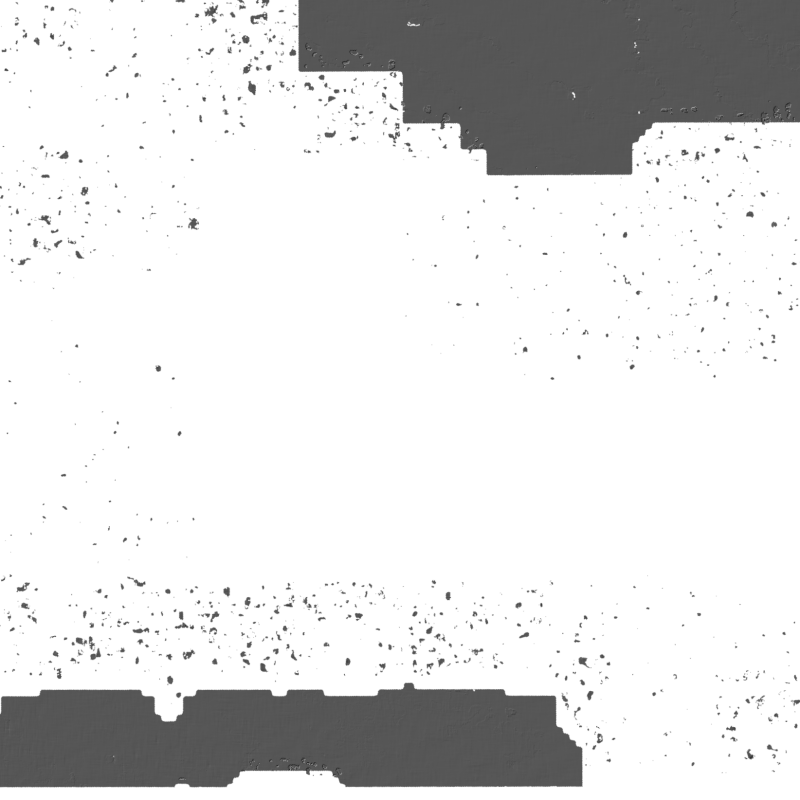
\includegraphics[width=3.0in]{images/examples/sparse_disp1.png}
  
\includegraphics[width=3.0in]{images/examples/sparse_disp3.png}
\caption{Example of a difficult flat terrain without (left) and with (right) using \texttt{sparse\_disp}.}
\label{fig:sparse-disp-example}
\end{figure}


\section{The Next Steps}

This tutorial described how to invoke \texttt{stereo} on Digital Globe
images, with and without map-projection, and how to handle other issues
specific to Digital Globe cameras and Earth data. We strongly suggest
you also study the tutorial about processing Mars imagery (chapter
\ref{ch:moc_tutorial}), starting with section \ref{running-stereo}, as it
has a wealth of information which we will not repeat here. In
particular, you will learn how to (a) customize the
\texttt{stereo.default} settings file, (b) use \texttt{point2dem} (with
the option \texttt{-r earth}) to create 3D terrain models, (c) visualize
the results, (d) align the obtained point clouds to another data source,
(e) perform 3D terrain adjustments in respect to a geoid, etc.

